\documentclass[11pt,professionalfonts,hyperref={pdftex,pdfpagemode=none,pdfstartview=FitH}]{beamer}
%\usepackage{times}
%\usefonttheme{serif}
%\usepackage{helvet}
%\usepackage{amsmath,amssymb}
\usepackage{graphicx,multirow}
\usepackage[scriptsize]{subfigure}
%\usepackage{movie15}

%\usepackage{warmread}
%\usepackage[all,import]{xy}

%\renewcommand\mathfamilydefault{\rmdefault}

\newcommand{\norm}[1]{\ensuremath{\left\| #1 \right\|}}
\newcommand{\bracket}[1]{\ensuremath{\left[ #1 \right]}}
\newcommand{\braces}[1]{\ensuremath{\left\{ #1 \right\}}}
\newcommand{\parenth}[1]{\ensuremath{\left( #1 \right)}}
\newcommand{\pair}[1]{\ensuremath{\langle #1 \rangle}}
\newcommand{\met}[1]{\ensuremath{\langle\langle #1 \rangle\rangle}}
\newcommand{\refeqn}[1]{(\ref{eqn:#1})}
\newcommand{\reffig}[1]{Fig. \ref{fig:#1}}
\newcommand{\tr}[1]{\mathrm{tr}\ensuremath{\negthickspace\bracket{#1}}}
\newcommand{\trs}[1]{\mathrm{tr}\ensuremath{[#1]}}
\newcommand{\deriv}[2]{\ensuremath{\frac{\partial #1}{\partial #2}}}
\newcommand{\SO}{\ensuremath{\mathsf{SO(3)}}}
\newcommand{\T}{\ensuremath{\mathsf{T}}}
\renewcommand{\L}{\ensuremath{\mathsf{L}}}
\newcommand{\so}{\ensuremath{\mathfrak{so}(3)}}
\newcommand{\SE}{\ensuremath{\mathsf{SE(3)}}}
\newcommand{\se}{\ensuremath{\mathfrak{se}(3)}}
\renewcommand{\Re}{\ensuremath{\mathbb{R}}}
\newcommand{\aSE}[2]{\ensuremath{\begin{bmatrix}#1&#2\\0&1\end{bmatrix}}}
\newcommand{\ase}[2]{\ensuremath{\begin{bmatrix}#1&#2\\0&0\end{bmatrix}}}
\newcommand{\D}{\ensuremath{\mathbf{D}}}
\newcommand{\Sph}{\ensuremath{\mathsf{S}}}
\renewcommand{\S}{\Sph}
\newcommand{\J}{\ensuremath{\mathbf{J}}}
\newcommand{\Ad}{\ensuremath{\mathrm{Ad}}}
\newcommand{\intp}{\ensuremath{\mathbf{i}}}
\newcommand{\extd}{\ensuremath{\mathbf{d}}}
\newcommand{\hor}{\ensuremath{\mathrm{hor}}}
\newcommand{\ver}{\ensuremath{\mathrm{ver}}}
\newcommand{\dyn}{\ensuremath{\mathrm{dyn}}}
\newcommand{\geo}{\ensuremath{\mathrm{geo}}}
\newcommand{\Q}{\ensuremath{\mathsf{Q}}}
\newcommand{\G}{\ensuremath{\mathsf{G}}}
\newcommand{\g}{\ensuremath{\mathfrak{g}}}
\newcommand{\Hess}{\ensuremath{\mathrm{Hess}}}
\newcommand{\refprop}[1]{Proposition \ref{prop:#1}}

\definecolor{mygray}{gray}{0.9}

\mode<presentation> {
  \usetheme{Warsaw}
  \usefonttheme{serif}
  \setbeamercovered{transparent}
}

\newcommand{\mypaper}{}

\setbeamertemplate{footline}%{split theme}
{%
  \leavevmode%
  \hbox{\begin{beamercolorbox}[wd=.7\paperwidth,ht=2.5ex,dp=1.125ex,leftskip=.3cm,rightskip=.3cm plus1fill]{author in head/foot}%
    \usebeamerfont{author in head/foot}\insertshorttitle
  \end{beamercolorbox}%
  \begin{beamercolorbox}[wd=.5\paperwidth,ht=2.5ex,dp=1.125ex,leftskip=.3cm,rightskip=.3cm]{title in head/foot}
    \usebeamerfont{title in head/foot}\mypaper\hfill \insertframenumber/\inserttotalframenumber
    \usebeamerfont{title in head/foot}\hfill \insertframenumber/\inserttotalframenumber
  \end{beamercolorbox}}%
  \vskip0pt%
} \setbeamercolor{box}{fg=black,bg=yellow}

\title[Bayesian Occupancy Grid Mapping via an Exact Inverse Sensor Model ]{\large Bayesian Occupancy Grid Mapping via an Exact Inverse Sensor Model}

\author{\vspace*{-0.3cm}}

\institute{\footnotesize
{\normalsize Evan Kaufman, Taeyoung Lee, \\Zhuming Ai, and Ira S. Moskowitz}\vspace*{0.2cm}\\
  Mechanical and Aerospace Engineering\\ George Washington University}

\date{}

\definecolor{tmp}{rgb}{0.804,0.941,1.0}
\setbeamercolor{numerical}{fg=black,bg=tmp}
\setbeamercolor{exact}{fg=black,bg=red}

\newtheorem{prop}{Proposition}



\renewcommand{\emph}[1]{\textit{\textbf{\color{blue}{#1}}}}


\begin{document}

\begin{frame}
  \titlepage
\end{frame}


\section*{}
\subsection*{Introduction}

\begin{frame}
\frametitle{Introduction}
\begin{itemize}
    \item Robotic Mapping
    \begin{itemize}
    	\item Goal: generate a map representing surrounding regions
	\item Crucial for simultaneous localization and mapping (SLAM) and autonomous exploration of uncertain environments
    	\item Popular mapping representations include \emph{occupancy grids}, octomaps, and feature-based maps
    \end{itemize}
\item Occupancy Grid Mapping
\begin{itemize}
	\item The environment may be decomposed into evenly spaced grid cells that are either \emph{occupied} or \emph{free}
	\item Probabilistic map: the goal is to obtain the \emph{probability} of each grid cell being occupied
\end{itemize}
\end{itemize}

\only<1->{
\begin{figure}
\centerline{
    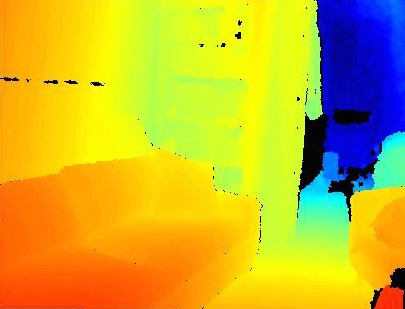
\includegraphics[height=2.1cm]{ogm_ex3.jpeg}\hspace*{0.1cm}
\hspace*{0.5cm}
    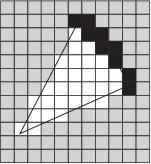
\includegraphics[height=2.1cm]{ogm_ex1.jpg}\hspace*{0.1cm}
\hspace*{0.5cm}
    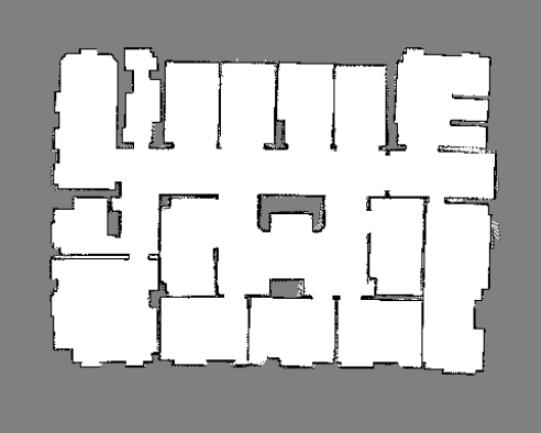
\includegraphics[height=2.1cm]{ogm_ex2.png}\hspace*{0.1cm}
}
\end{figure}}

\end{frame}


\begin{frame}
\frametitle{Introduction}
\framesubtitle{Problem Definition}

\begin{itemize}
	\item The Map and the Robot
	\begin{itemize}
	\item Map $m$ is composed of $n_m$ grid cells with known location and size
	\item The $i$-th grid cell $\mathbf{m}_i$ is a \emph{static binary} random variable, independent of other grid cells: $P(m)=P(\mathbf{m}_1,\mathbf{m}_2,\ldots,\mathbf{m}_{n_m})=\prod_{i=1}^{n_m}P(\mathbf{m}_i)$
	\item \emph{Pose} $X_t$ is known, containing robot \emph{position} and \emph{attitude}
	\end{itemize}
\vspace*{0.0cm}\pause
\end{itemize}
\begin{minipage}[t]{7.0cm}
\begin{itemize}
	\item Depth Measurements
	\begin{itemize}
	\item Each measurement origin and direction is known \emph{deterministically}
	\item A measurement \emph{scan} $Z_t=\braces{z_{t,1},z_{t,2},\ldots,z_{t,n_z}}$ contains $n_z$ measurement \emph{rays} (depths)% at the $t$-th time step, and the history of measurement scans $Z_{1:t}$ is known
\item The \emph{forward sensor model} is known from the sensor properties
\end{itemize}
\end{itemize}
\end{minipage}
\begin{minipage}[t]{3.0cm}
%The \emph{forward sensor model} is the probability density distribution $p(z_{t,l}|m,X_{t})$  known from the sensor properties
\hspace*{0.25cm}
\begin{figure}[!htbp]
\vspace*{-0.25cm}
%\vspace*{0.25cm}
\centerline{
    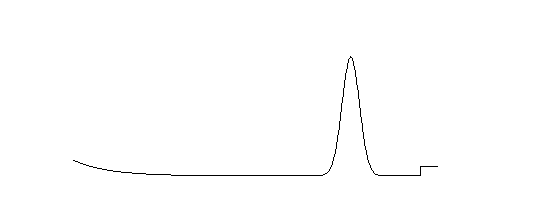
\includegraphics[width=3.5cm]{BeamModel.png}\hspace*{0.1cm}
    }
\vspace*{0.25cm}
\centerline{
    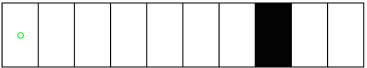
\includegraphics[width=2.5cm]{1D_True_Grid.png}\hspace*{0.1cm}
%    \hspace*{0.75cm}
    }
{Beam Model for Range Finders}
\end{figure}

\end{minipage}



\end{frame}

\begin{frame}
\frametitle{Introduction}
\framesubtitle{Problem Definition}

\begin{itemize}
	\item Bayesian Framework
	\begin{itemize}
	\item Markov Assumption: latest a priori cell occupancy probabilities capture the information from all prior observations
	\item Log-Odds Ratio: popular representation due to simple additive update structure and probability truncation avoidance, but requires the \emph{assumption}
	\begin{align*}
		P(Z_t|\mathbf{m}_i,X_{1:t},Z_{1:t-1})\approx P(Z_t|\mathbf{m}_i,X_t)
	\end{align*}
	\end{itemize}
\vspace*{0.0cm}\pause
	\item Inverse Sensor Model
	\begin{align*}
&P(\mathbf{m}_i|z_{t,l},X_{1:t},Z_{1:t-1})\nonumber
\\
&=\eta_{t,l}\sum_{m\in\mathcal{M}_i}p(z_{t,l}|m,X_{t})P(m|X_{1:t-1},Z_{1:t-1}).
\end{align*}
	\begin{itemize}
	\item Given $n$ grid cells: $\mathcal O(2^n)$ is \emph{computationally intractable}, motivating a different solution
	\end{itemize}
\end{itemize}

\end{frame}

\begin{frame}
\frametitle{Introduction}
\framesubtitle{Problem Definition}

\begin{minipage}[t]{7.0cm}
\begin{itemize}
	\item Approximate a function for the inverse sensor model based on intuition
	\begin{itemize}
		\item Simple to implement, but mathematically inaccurate
	\end{itemize}
\end{itemize}
\end{minipage}
\begin{minipage}[t]{3.0cm}
\begin{figure}[!htbp]
\centerline{
    \vspace*{-0.5cm}
%	\hspace*{0.25cm}
    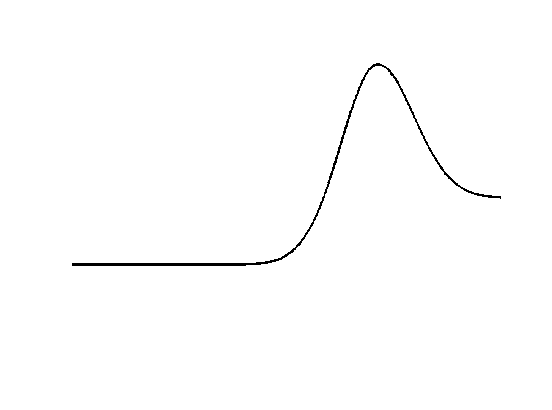
\includegraphics[width=4.0cm]{Approx_ISM_shortened.png}\hspace*{0.1cm}
    }
\centerline{
    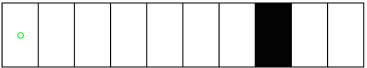
\includegraphics[width=3.5cm]{1D_True_Grid.png}
%    \hspace*{0.75cm}
    }
		\end{figure}
\end{minipage}
\vspace*{-0.5cm}
\begin{itemize}
	\item Find a solution through learning
	\begin{itemize}
		\item Simulate maps, poses, and measurements and use learning to obtain an inverse sensor model
		\item Complicated, unclear how these parameters are chosen
	\end{itemize}
	\item Goal: design a \emph{simple} and \emph{accurate} occupancy grid mapping method avoiding log-odds ratio assumptions
\end{itemize}
%
%	\begin{minipage}[width=1cm]
%		Approximate a function for the inverse sensor model based on intuition
%	\end{minipage}
%	\begin{minipage}[width=1cm]
%		Approximate a function for the inverse sensor model based on intuition2
%	\end{minipage}
%\begin{itemize}
%	\item Heuristic Approach
%	\begin{itemize}
%	\item asdf
%\begin{figure}
%\centerline{
%    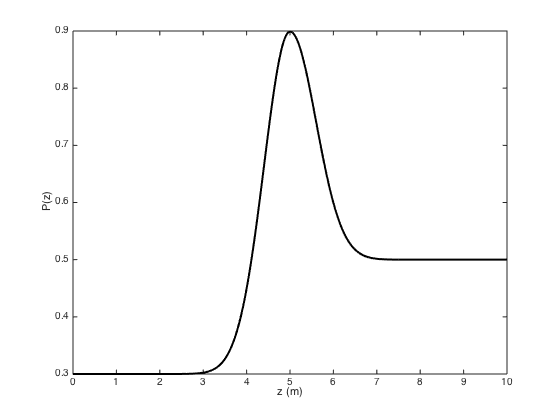
\includegraphics[width=3.5cm]{ISM_Approx_Single_Ray.png}\hspace*{0.1cm}
%    }
%\centerline{
%    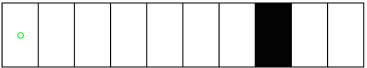
\includegraphics[width=3.5cm]{1D_True_Grid.png}\hspace*{0.1cm}
%%    \hspace*{0.75cm}
%    }
%\end{figure}
%	\item Simple to implement, but mathematically inaccurate
%	\end{itemize}
%\vspace*{0.3cm}\pause
%\begin{itemize}
%	\item Learning
%	\begin{itemize}
%	\item Idea
%	\item Complicated, not clear how parameters are chosen
%	\end{itemize}
%\vspace*{0.3cm}\pause
%	\item Goal: design a simple and accurate method for occupancy grid mapping that avoids log-odds ratio assumptions
%\end{itemize}

\end{frame}


\section*{}
\subsection*{Probabilistic Mapping}



\begin{frame}
\frametitle{Single Measurement Ray}

\begin{itemize}
    \item Main idea: make use of occupancy grid mapping \emph{assumptions} and extract \emph{patterns} from probabilistic properties to find a \emph{computationally-efficient} solution
	\begin{itemize}
		\item Since the origin and direction of each measurement ray is known deterministically, the set of grid cells that the ray intersects is \emph{known through geometry}
		\item A depth reading follows the forward sensor model, which \emph{only depends} on the first occupied grid cell along the measurement ray
	\end{itemize}
\end{itemize}
\setcounter{subfigure}{0}
\begin{figure}[!htbp]
\vspace*{-0.25cm}
\centerline{
	\subfigure[True Grid]{
	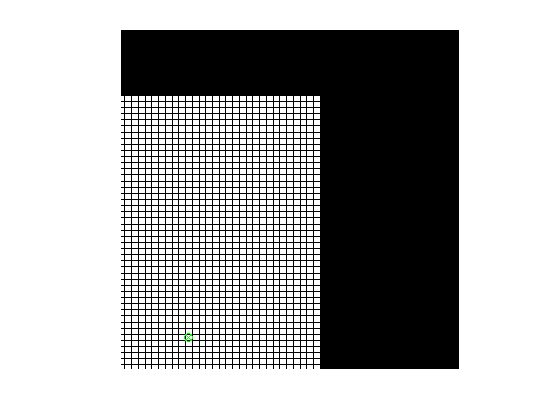
\includegraphics[width=4.0cm]{simple_true_grid.png}\hspace*{-0.5cm}}
	\subfigure[Probabilistic Map]{
	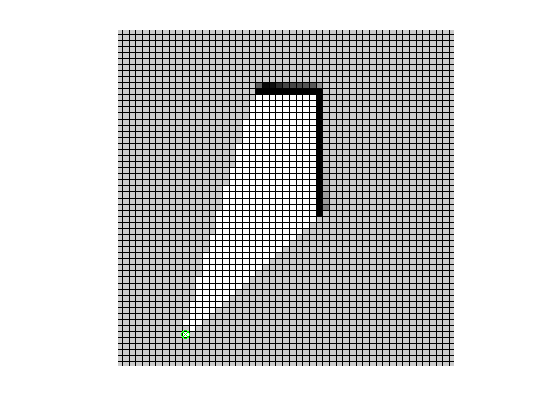
\includegraphics[width=4.0cm]{simple_sweep.png}}
 }
\end{figure}
\end{frame}




\begin{frame}
\frametitle{Single Measurement Ray}

\begin{itemize}
    \item Reduced Map
	\begin{itemize}
		\item Consider a reduced map of the $l$-th measurement ray, namely $r_l=\braces{\mathbf{r}_{l,1},\mathbf{r}_{l,2},\ldots,\mathbf{r}_{l,n_{r,l}}}$, consisting of grid cells \emph{intersected} by the measurement ray within the sensor limits, \emph{indexed by increasing distance}
		\item Since reduced map $r_l$ is composed of binary random variables, it has \emph{$2^{n_{r,l}}$} possible solutions
		\item If $\mathbf{r}_{l,1}$ is occupied (a priori probability $P(\mathbf{r}_{l,1}|X_{1:t-1},Z_{1:t-1})$), then each occupancy $\mathbf{r}_{l,2:n_{r,l}}$ does \emph{not} affect forward sensor model $P(z_{t,l}|\mathbf{r}_{l,1},X_t)$
		\item Similarly, if $\mathbf{r}_{l,2}$ is occupied (a priori probability $P(\bar{\mathbf{r}}_{l,1}|X_{1:t-1},Z_{1:t-1})P(\mathbf{r}_{l,2}|X_{1:t-1},Z_{1:t-1})$), then forward sensor model $P(z_{t,l}|\mathbf{r}_{l,2},X_t)$ is independent of grid cells of higher index
		\item This concept is extended for all grid cells in $r_l$
	\end{itemize}
\end{itemize}
\end{frame}

\begin{frame}
\frametitle{Single Measurement Ray}

\begin{itemize}
	\item Define $P(\mathbf{r}_{l,k}|z_{t,l},X_{1:t},Z_{1:t-1})=\eta_{t,l}\tilde P(\mathbf{r}_{l,k}|z_{t,l},X_{1:t},Z_{1:t-1})$ and its complement $P(\bar{\mathbf{r}}_{l,k}|z_{t,l},X_{1:t},Z_{1:t-1})=1-P(\mathbf{r}_{l,k}|z_{t,l},X_{1:t},Z_{1:t-1})=\eta_{t,l}\tilde P(\bar{\mathbf{r}}_{l,k}|z_{t,l},X_{1:t},Z_{1:t-1})$
	\item The $k$-th unnormalized probability is written generally as
	\begin{align*}
		& \tilde P(\mathbf{r}_{l,k}|z_{t,l},X_{1:t},Z_{1:t-1})\nonumber\\
		&=P(\mathbf{r}_{l,k}|X_{1:t-1},Z_{1:t-1})\nonumber\times 
		\bigg[\sum_{i=1}^{k-1}\bigg\{\prod_{j=0}^{i-1}P(\bar{\mathbf{r}}_{l,j}|X_{1:t-1},Z_{1:t-1})\bigg\}\nonumber\\
		&\quad\times p(z_{t,l}|\mathbf{r}_{l,i+},X_t)P(\mathbf{r}_{l,i}|X_{1:t-1},Z_{1:t-1})\bigg]\nonumber\\
		&\quad + \bigg\{\prod_{j=0}^{k-1}P(\bar{\mathbf{r}}_{l,j}|X_{1:t-1},Z_{1:t-1})\bigg\}\nonumber\\
		&\quad\times p(z_{t,l}|\mathbf{r}_{l,k+},X_t)P(\mathbf{r}_{l,k}|X_{1:t-1},Z_{1:t-1})
	\end{align*}
\end{itemize}
\end{frame}

\begin{frame}
\frametitle{Single Measurement Ray}

\begin{itemize}
	\item The unnormalized complement $\tilde P(\bar{\mathbf{r}}_{l,k}|z_{t,l},X_{1:t},Z_{1:t-1})$ takes a similar form
	\item Because $P(\mathbf{r}_{l,k}|z_{t,l},X_{1:t},Z_{1:t-1})+P(\bar{\mathbf{r}}_{l,k}|z_{t,l},X_{1:t},Z_{1:t-1})=1$, the normalizer is
	\begin{align*}
		\eta_{t,l}&=
		\bigg[\sum_{i=1}^{n_{r,l}+1}\bigg\{\prod_{j=0}^{i-1}P(\bar{\mathbf{r}}_{l,j}|X_{1:t-1},Z_{1:t-1})\bigg\}\nonumber\\
		&\quad\times p(z_{t,l}|\mathbf{r}_{l,i+},X_t)P(\mathbf{r}_{l,i}|X_{1:t-1},Z_{1:t-1})\bigg]^{-1}
	\end{align*}
\end{itemize}
\end{frame}

\begin{frame}
\frametitle{Single Measurement Ray}

\begin{itemize}
	\item Computational Efficiency
	\begin{itemize}
		\item Several of the terms required for $\eta_{t,l}$ and $\tilde P(\mathbf{r}_{l,k}|z_{t,l},X_{1:t},Z_{1:t-1})$ for each $k=1,2,\ldots,n_{r,l}$ are repeated and need not be computed more than once
		\item \emph{Computational order $\mathcal O(n_{r,l}+1)$} for all grid cells in reduced map $r$: each grid cell once and the empty map case
		\item Analytic solution is valid for any forward sensor model dependent on the closest occupied space
	\end{itemize}
\pause
	\item Comparison to other approaches
	\begin{itemize}
		\item It is commonly believed that the computational order is $\mathcal O(2^{n_{r,l}})$; the proposed method is \emph{$2^{n_{r,l}}\left(\frac{n_{r,l}}{n_{r,l}+1}\right)$ times faster} for the \emph{same solution}
		\item Proposed method completely avoids inaccuracies associated with heuristic solutions, learned methods, and log-odds ratio update assumptions
	\end{itemize}
\end{itemize}
\end{frame}


\begin{frame}
\frametitle{Full Measurement Scan}

\begin{itemize}
	\item Two Methods
	\begin{itemize}
		\item \emph{Ray-By-Ray Inverse Sensor Model}: each measurement ray is evaluated individually for updating the map
		\item \emph{Synergistic Scan Inverse Sensor Model}: all measurement rays are evaluated simultaneously
	\end{itemize}
\end{itemize}

\end{frame}


\begin{frame}
\frametitle{Ray-By-Ray Inverse Sensor Model}

\begin{itemize}
	\item Main idea: given a scan of measurement rays, update the map based on each measurement ray \emph{individually} and \emph{sequentially}
	\item Conditional probability:
	\begin{align*}
		P(\mathbf{m}_i|X_{1:t}&,Z_{1:t})\nonumber\\&
		=P((\dots(((\mathbf{m}_i|X_{1:t},Z_{1:t-1})|z_{t,1})|z_{t,2})|\ldots)|z_{t,n_z})
	\end{align*}
	\item Benefit: the measurement rays maintain some dependency as they capture the same map
	\item Drawback: the best order for evaluating rays is not necessarily chosen
\end{itemize}

\end{frame}

\begin{frame}
\frametitle{Synergistic Scan Inverse Sensor Model}

\begin{itemize}
	\item Main idea: consider every measurement ray inside a scan \emph{simultaneously} to update all grid cells inside the FOV
	\item Probability derived from a Bayesian approach:
	\begin{align*}
		P(\mathbf{m}_i|X_{1:t},Z_{1:t})
		&=\xi_i P(\mathbf{m}_i|{X_{1:t-1}},Z_{1:t-1})\nonumber\\&\quad\times
		\prod_{l\in\mathcal L_i}
		\hat P(\mathbf{r}_{l,k}|z_{t,l},X_{1:t},Z_{1:t-1}),
		\\
		\hat P(\mathbf{r}_{l,k}|z_{t,l},X_{1:t},Z_{1:t-1})&
		\triangleq \frac{\tilde P(\mathbf{r}_{l,k}|z_{t,l},X_{1:t},Z_{1:t-1})}{P(\mathbf{m}_i|X_{1:t-1},Z_{1:t-1})}
	\end{align*}
	\item Benefit: synergistic update provides a method where all rays are considered simultaneously
	\item Drawback: required assumption that the measurement rays are independent, though they capture the same map
\end{itemize}

\end{frame}


\section*{}
\subsection*{Results}

\begin{frame}
\frametitle{Numerical Example}

\begin{itemize}
\item The proposed occupancy grid mapping algorithm and a heuristic solution are compared in a simulated scenario where a robot moves around a closed room
\begin{figure}
\vspace*{0.2cm}
\centerline{
\subfigure[Exact Proposed Occupancy Grid Mapping]{
	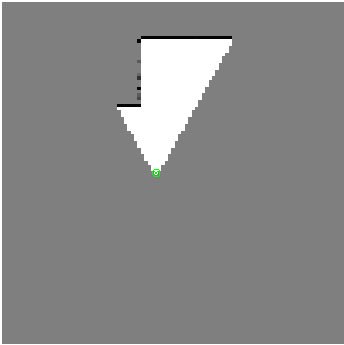
\includegraphics[width=1.5cm]{Compare_ISM_1.png}\hspace*{0.1cm}
	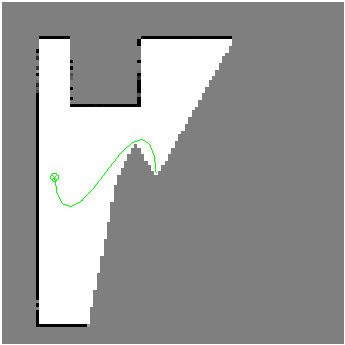
\includegraphics[width=1.5cm]{Compare_ISM_2.png}\hspace*{0.1cm}
	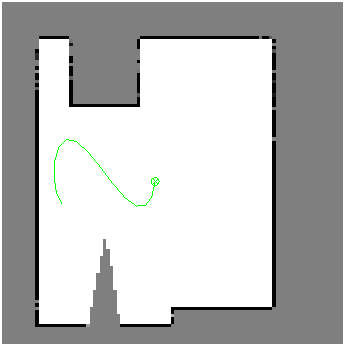
\includegraphics[width=1.5cm]{Compare_ISM_3.png}\hspace*{0.1cm}
	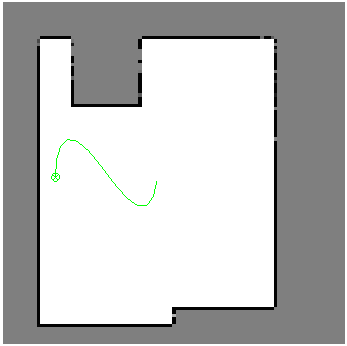
\includegraphics[width=1.5cm]{Compare_ISM_4.png}\hspace*{0.1cm}
	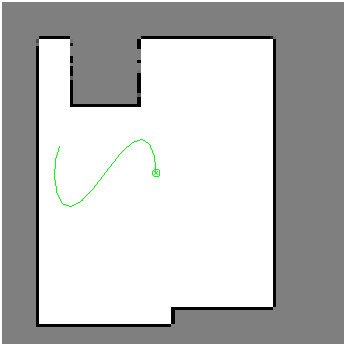
\includegraphics[width=1.5cm]{Compare_ISM_5.png}\hspace*{0.1cm}
	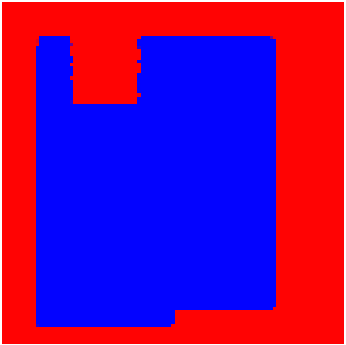
\includegraphics[width=1.5cm]{Compare_ISM_H.png}
	}}
\vspace*{0.2cm}
\centerline{
\subfigure[Heuristic Occupancy Grid Mapping]{
	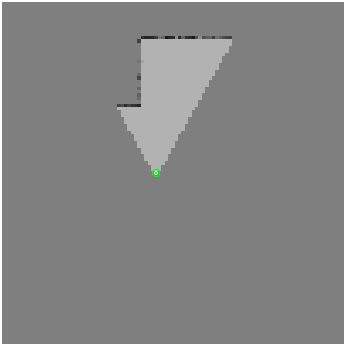
\includegraphics[width=1.5cm]{Compare_Approx_1.png}\hspace*{0.1cm}
	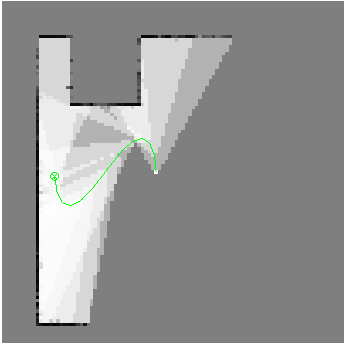
\includegraphics[width=1.5cm]{Compare_Approx_2.png}\hspace*{0.1cm}
	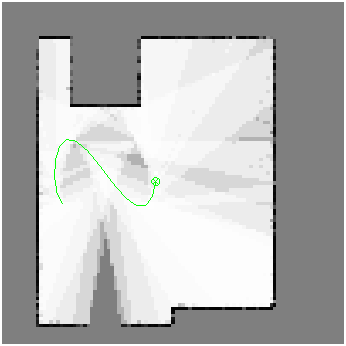
\includegraphics[width=1.5cm]{Compare_Approx_3.png}\hspace*{0.1cm}
	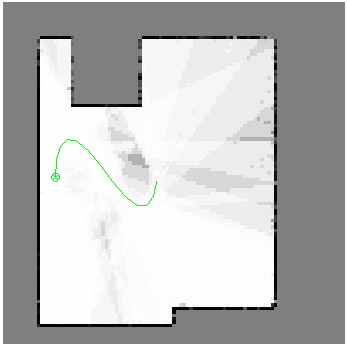
\includegraphics[width=1.5cm]{Compare_Approx_4.png}\hspace*{0.1cm}
	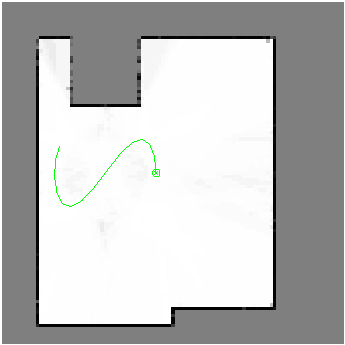
\includegraphics[width=1.5cm]{Compare_Approx_5.png}\hspace*{0.1cm}
	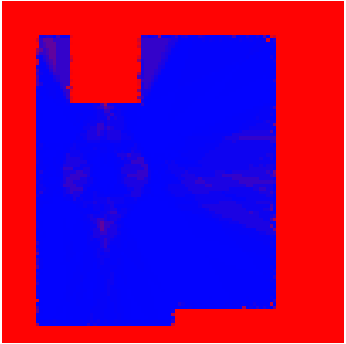
\includegraphics[width=1.5cm]{Compare_Approx_H.png}
	}}
\end{figure}
\item The robot trajectory and the same set of measurements are used with both approaches
\end{itemize}

\end{frame}



\begin{frame}
\frametitle{Experimental Example}

\begin{itemize}
\item Kinect is placed under a desk and receives a single measurement scan
\setcounter{subfigure}{0}
\begin{figure}[!htbp]
\centerline{
\vspace*{0.5cm}
		\subfigure[Test Setup]{
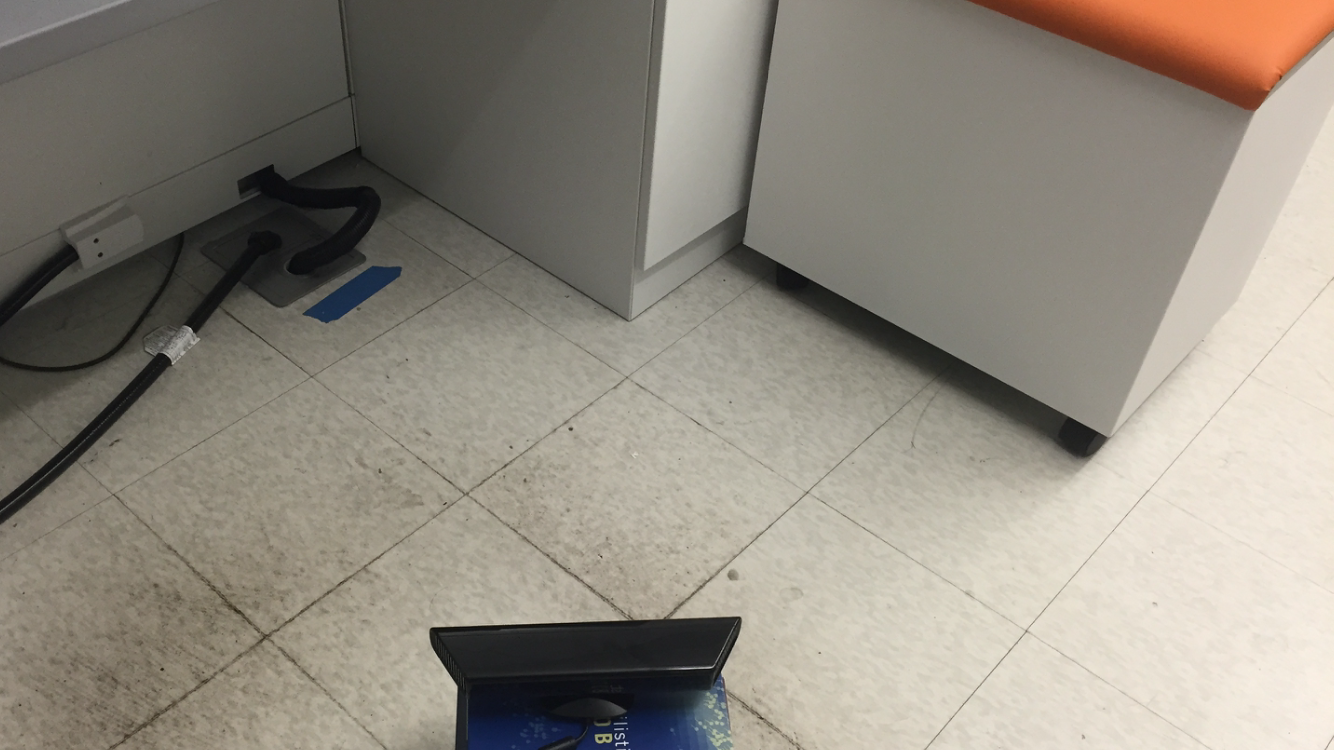
\includegraphics[height=1.5cm]{TestSetup.png}\hspace*{0.5cm}}
		\subfigure[Camera View]{
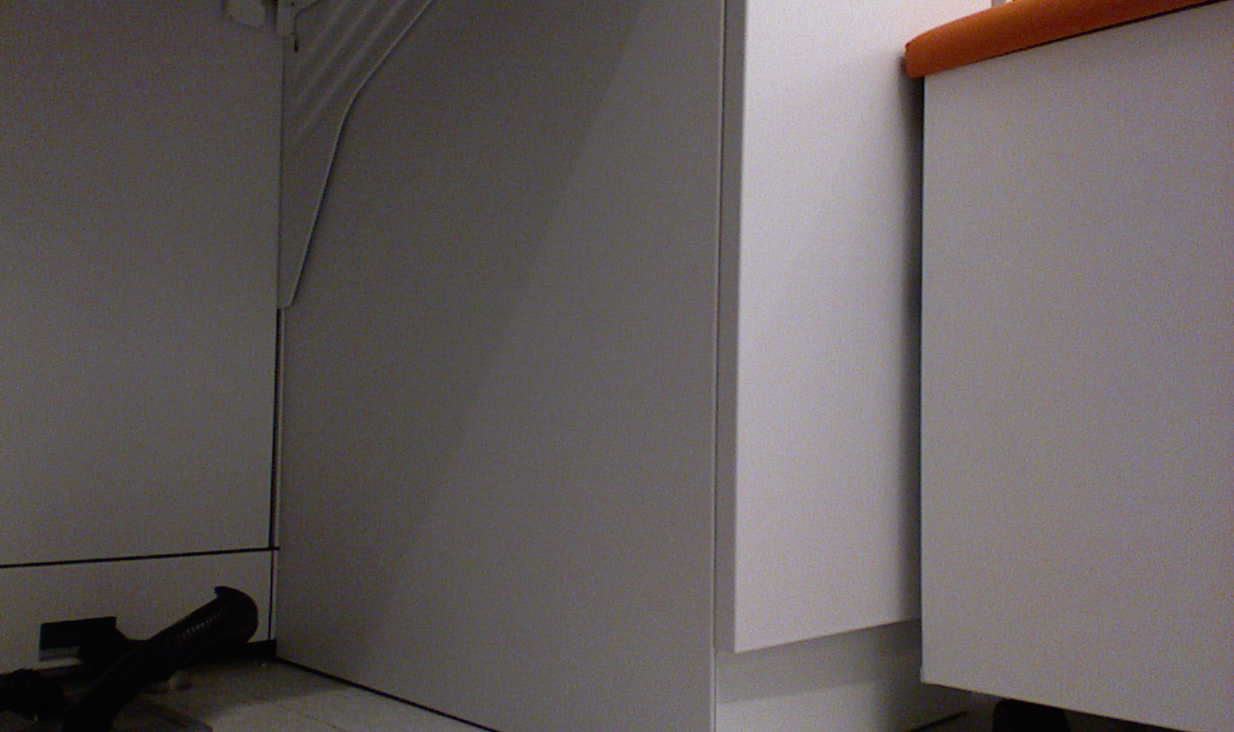
\includegraphics[height=1.5cm]{KinectView.png}}}
\end{figure}
\vspace{-0.5cm}\pause
\item Exact and approximate inverse sensor models are compared
\end{itemize}
\setcounter{subfigure}{0}
\begin{figure}[!htbp]
	\centerline{
		\subfigure[Exact \newline \hspace*{0.4cm} Occupancy]{
\includegraphics[height=2.1cm]{KinectDeskISM.png}}\hspace*{0.3cm}
		\subfigure[Exact \newline \hspace*{0.4cm} Uncertainty]{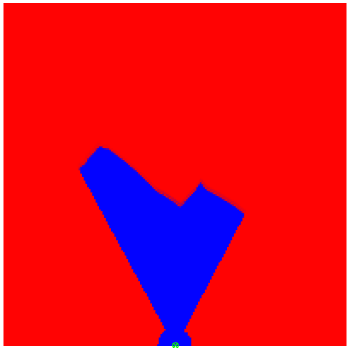
\includegraphics[height=2.1cm]{KinectDeskISM_H.png}}\hspace*{0.3cm}
		\subfigure[Approx. \newline \hspace*{0.4cm} Occupancy]{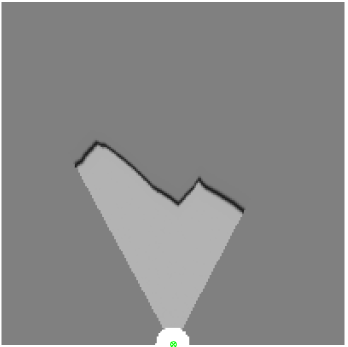
\includegraphics[height=2.1cm]{KinectDeskApprox.png}}\hspace*{0.3cm}
		\subfigure[Approx. \newline \hspace*{0.4cm} Uncertainty]{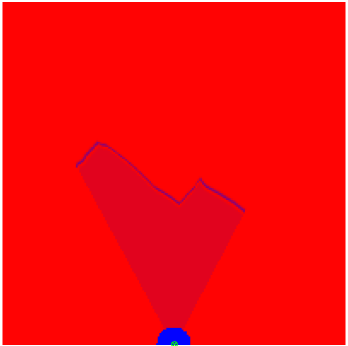
\includegraphics[height=2.1cm]{KinectDeskApprox_H.png}}
		}
\end{figure}


\end{frame}





\begin{frame}
\frametitle{Numerical Example}

\begin{itemize}
\item Similar concepts are extended to autonomous exploration
\item The poses are chosen to maximize map information gain
\setcounter{subfigure}{0}
\begin{figure}
\vspace*{0.2cm}
\centerline{
	\subfigure[$t=1$ sec]{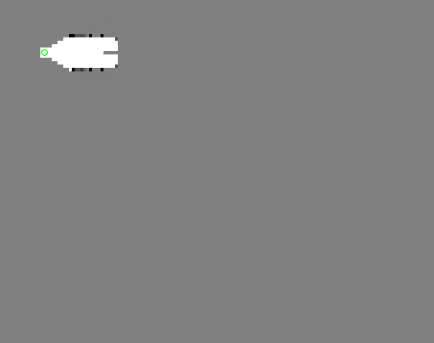
\includegraphics[width=3.0cm]{RDShowcaseMotionPlanning1sec.png}}\hspace*{0.2cm}
	\subfigure[$t=100$ sec]{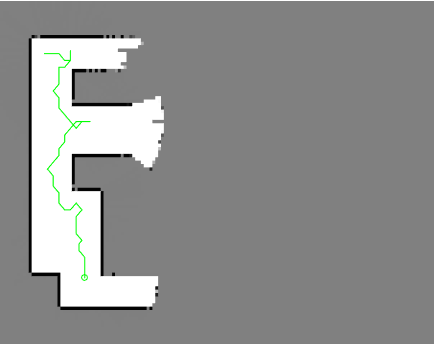
\includegraphics[width=3.0cm]{RDShowcaseMotionPlanning100sec.png}}\hspace*{0.2cm}
	\subfigure[$t=200$ sec]{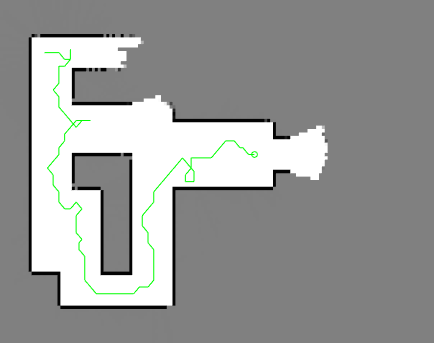
\includegraphics[width=3.0cm]{RDShowcaseMotionPlanning200sec.png}}
	}
\vspace*{0.0cm}
\centerline{
	\subfigure[$t=300$ sec]{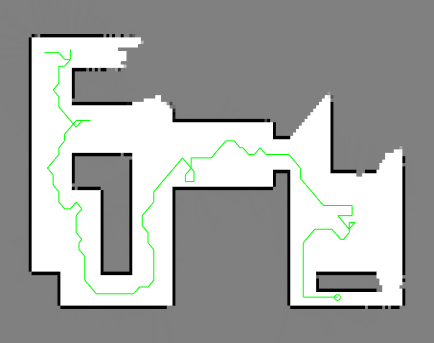
\includegraphics[width=3.0cm]{RDShowcaseMotionPlanning300sec.png}}\hspace*{0.2cm}
	\subfigure[$t=400$ sec]{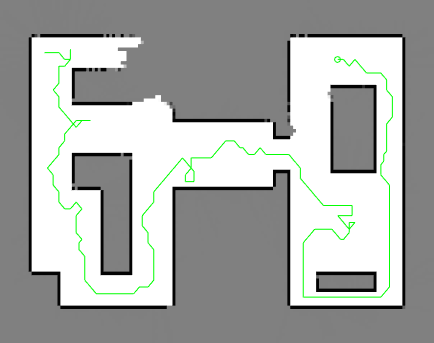
\includegraphics[width=3.0cm]{RDShowcaseMotionPlanning400sec.png}}\hspace*{0.2cm}
	\subfigure[$t=500$ sec]{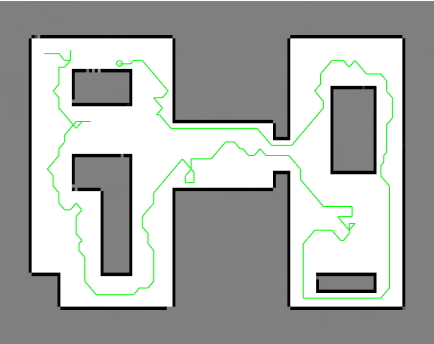
\includegraphics[width=3.0cm]{RDShowcaseMotionPlanning500sec.png}}
	}
\end{figure}
\end{itemize}

\end{frame}





\section*{}
\subsection*{Conclusions and Future Work}

\begin{frame}
\frametitle{Conclusions}
\begin{itemize}
        	\item Proposed an occupancy grid mapping technique that uses the \emph{exact probabilistic solution}
	\item Computational cost is reduced \emph{substantially} for \emph{real-time implementation} using probabilisitic properties and exploiting mathematical patterns
	\item Assumptions required for log-odds ratio Bayesian updating are avoided
	\item The proposed technique is compared with a heuristic solution to show the improvement in algorithm performance 
\end{itemize}
\end{frame}


\begin{frame}
\frametitle{Current and Future Work}
\begin{itemize}
    \item Current Reseach
    \begin{itemize}
        	\item Using the normalizer from this research, a method to \emph{predict map information gain} governs an \emph{autonomous exploration} algorithm
	\item Both the mapping and autonomous exploration algorithms are successfully tested with C++ ROS nodes
	\item We are completing ground vehicle tests where a robot autonomously explores a room
    \end{itemize}
    \item Future Work
    \begin{itemize}
        	\item Apply occupancy grid mapping and autonomous exploration in a \emph{3D} setting with a \emph{flying robot}
	\item Extend problem to \emph{multiple vehicles} for exploring uncertain spaces
    \end{itemize}
\end{itemize}
\end{frame}




\end{document}

